\section{Testing}
\label{sect:testing}

	As a distributed topology in a Big-Data environment could be a complex structure, testing is (as always) no marginal problem. In our Storm based scenario, we have Spouts that are emitting the initial input into the topology, Bolts that are executing operations on that input in one or several chains of neighbouring Bolts and we have the topology that combines Spouts and Bolt chains with each other to form a structure, which is able to solve a specific Big-Data analytics problem. 
	In such a scenario, it is not easy to find and solve problems and errors, as monitoring is only in place for the whole topology and not for each individual element. Additionally, a Storm topology is only debuggable at runtime, which makes it quite hard to find bugs or \textit{at least just realize that the topology is not working as expected} for large setups. 
	To find problems and errors in such a setup several points of view are needed to be addressed in order to find the source of a problem faster and more reliable as it would usually be the case.
	
\subsection{Test-Suite Approach}
	In order to cope with the challenges of testing in complex and distributed Storm environments, we developed our own Test-Suite, which focuses on three different levels that may contain, combined with each other, the most common problem sources in an instance of one of our CIT-Storm topologies. The three different problem levels that we considered of importance were the following ones, sorted by abstraction level in the topology:
	
	\begin{description}
	 \descriptor{Operator-Tests}
		Are describing the validity of a specific user defined function that is caring about the input tuple execution inside a Bolt. For a well defined testing setup, each Bolt inside the testing topology should have an Operator- \& a Bolt-Test (described beneath) to fully assure that the respective Bolt is behaving as expected \textit{without any outside influences}, namely predecessor Bolts that are sending unexpected input to this Bolt. An Operator-Test is thus using pre-defined tuple input and checks if the asserted output of the operator to be tested is matching with the factual output.
		\begin{center}
			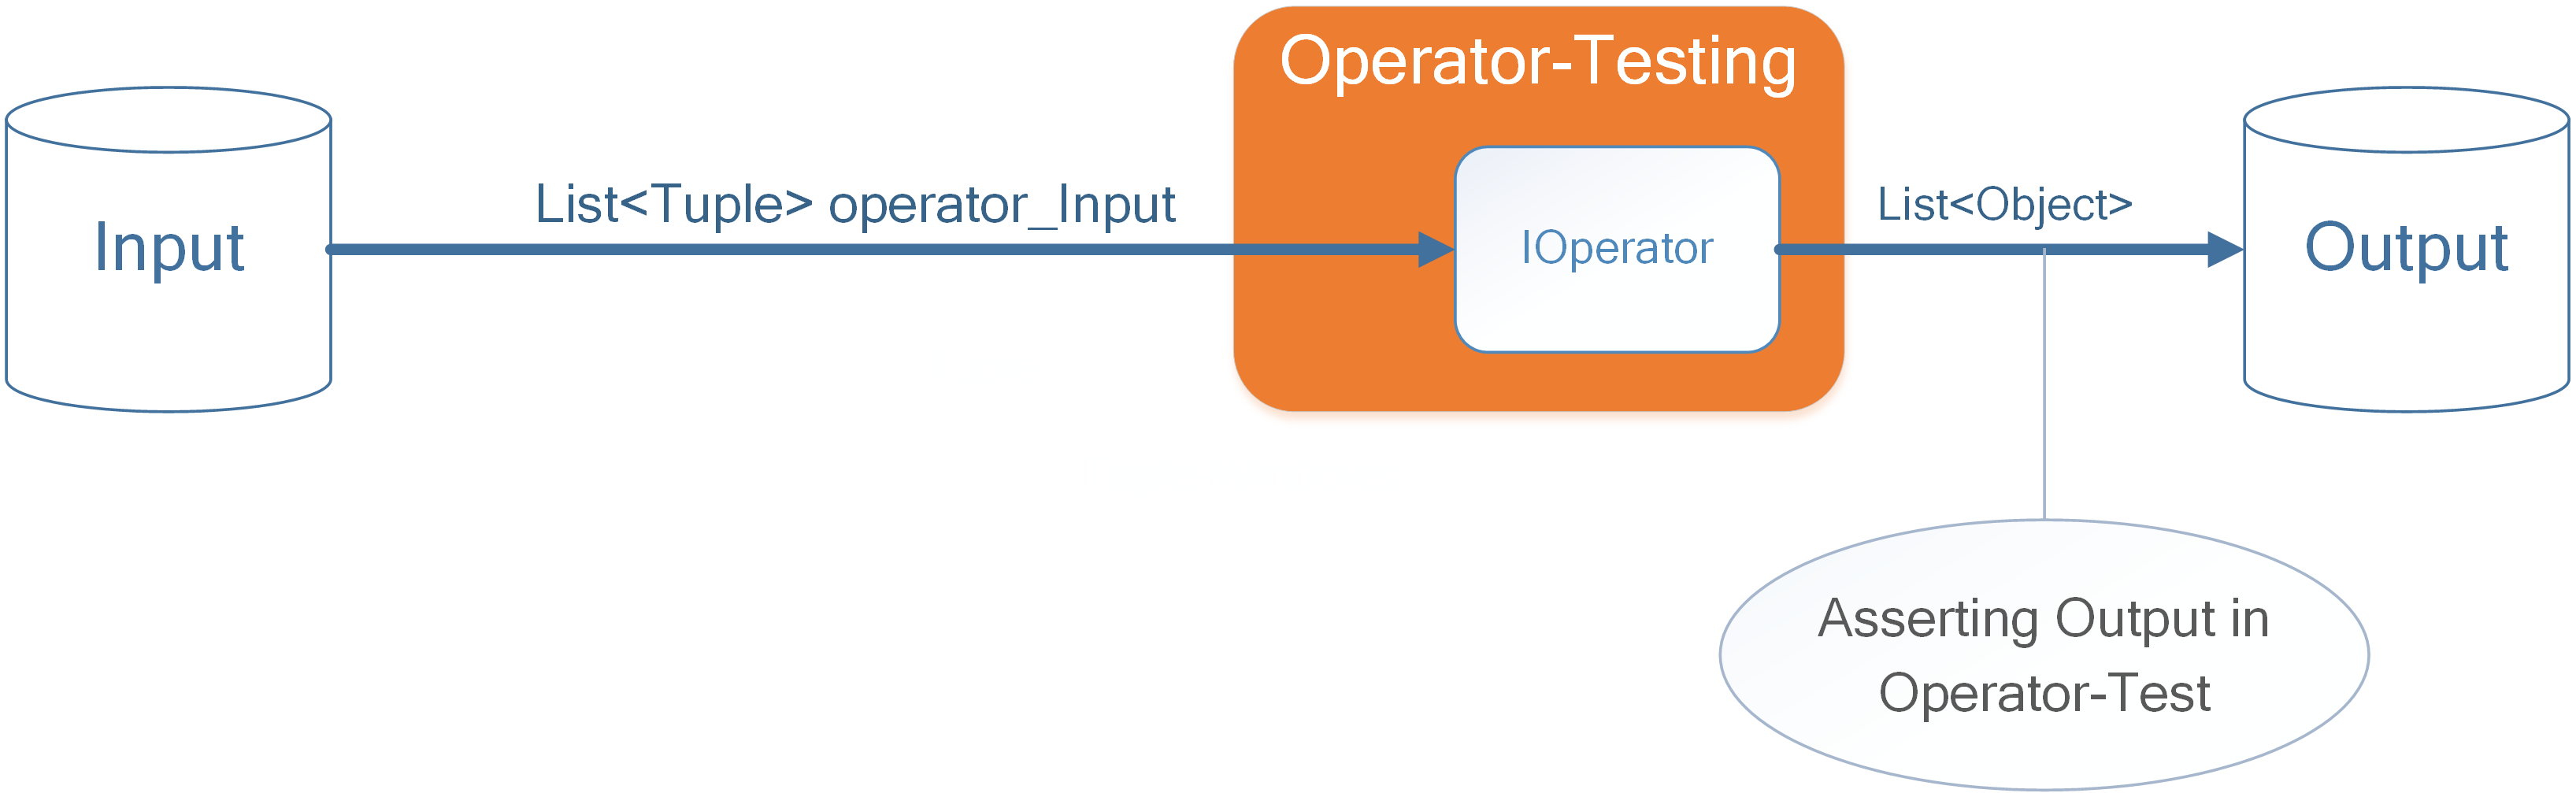
\includegraphics[width=0.4\textwidth]{./images/08_testing/OperatorTests.png}
		\end{center}

		
	 \descriptor{Bolt-Tests}
		Are combining Operator-Tests with additional Window-Handling, as needed to build streaming input execution. In our CIT-Storm implementation (as defined in \ref{sect:udfBolt}), we are using \textit{Time-} or \textit{Count-Windows} to wait a specific time or for a specific amount of input tuples, until the execution of those input tuples will be passed to the Operator. \\
		In perspective if this Testing-Suite, the Operator-Test (which was already successfully executed before) is only returning the correctness of a given input, relative to an asserted output, whereas a Bolt-Test includes testing with focus on the used window and its output after a \texttt{window.flush()}. The Bolt-Test will only be successful when a window returns the expected tuples after a given time and the Operator will correctly handle this input.
		\begin{center}
			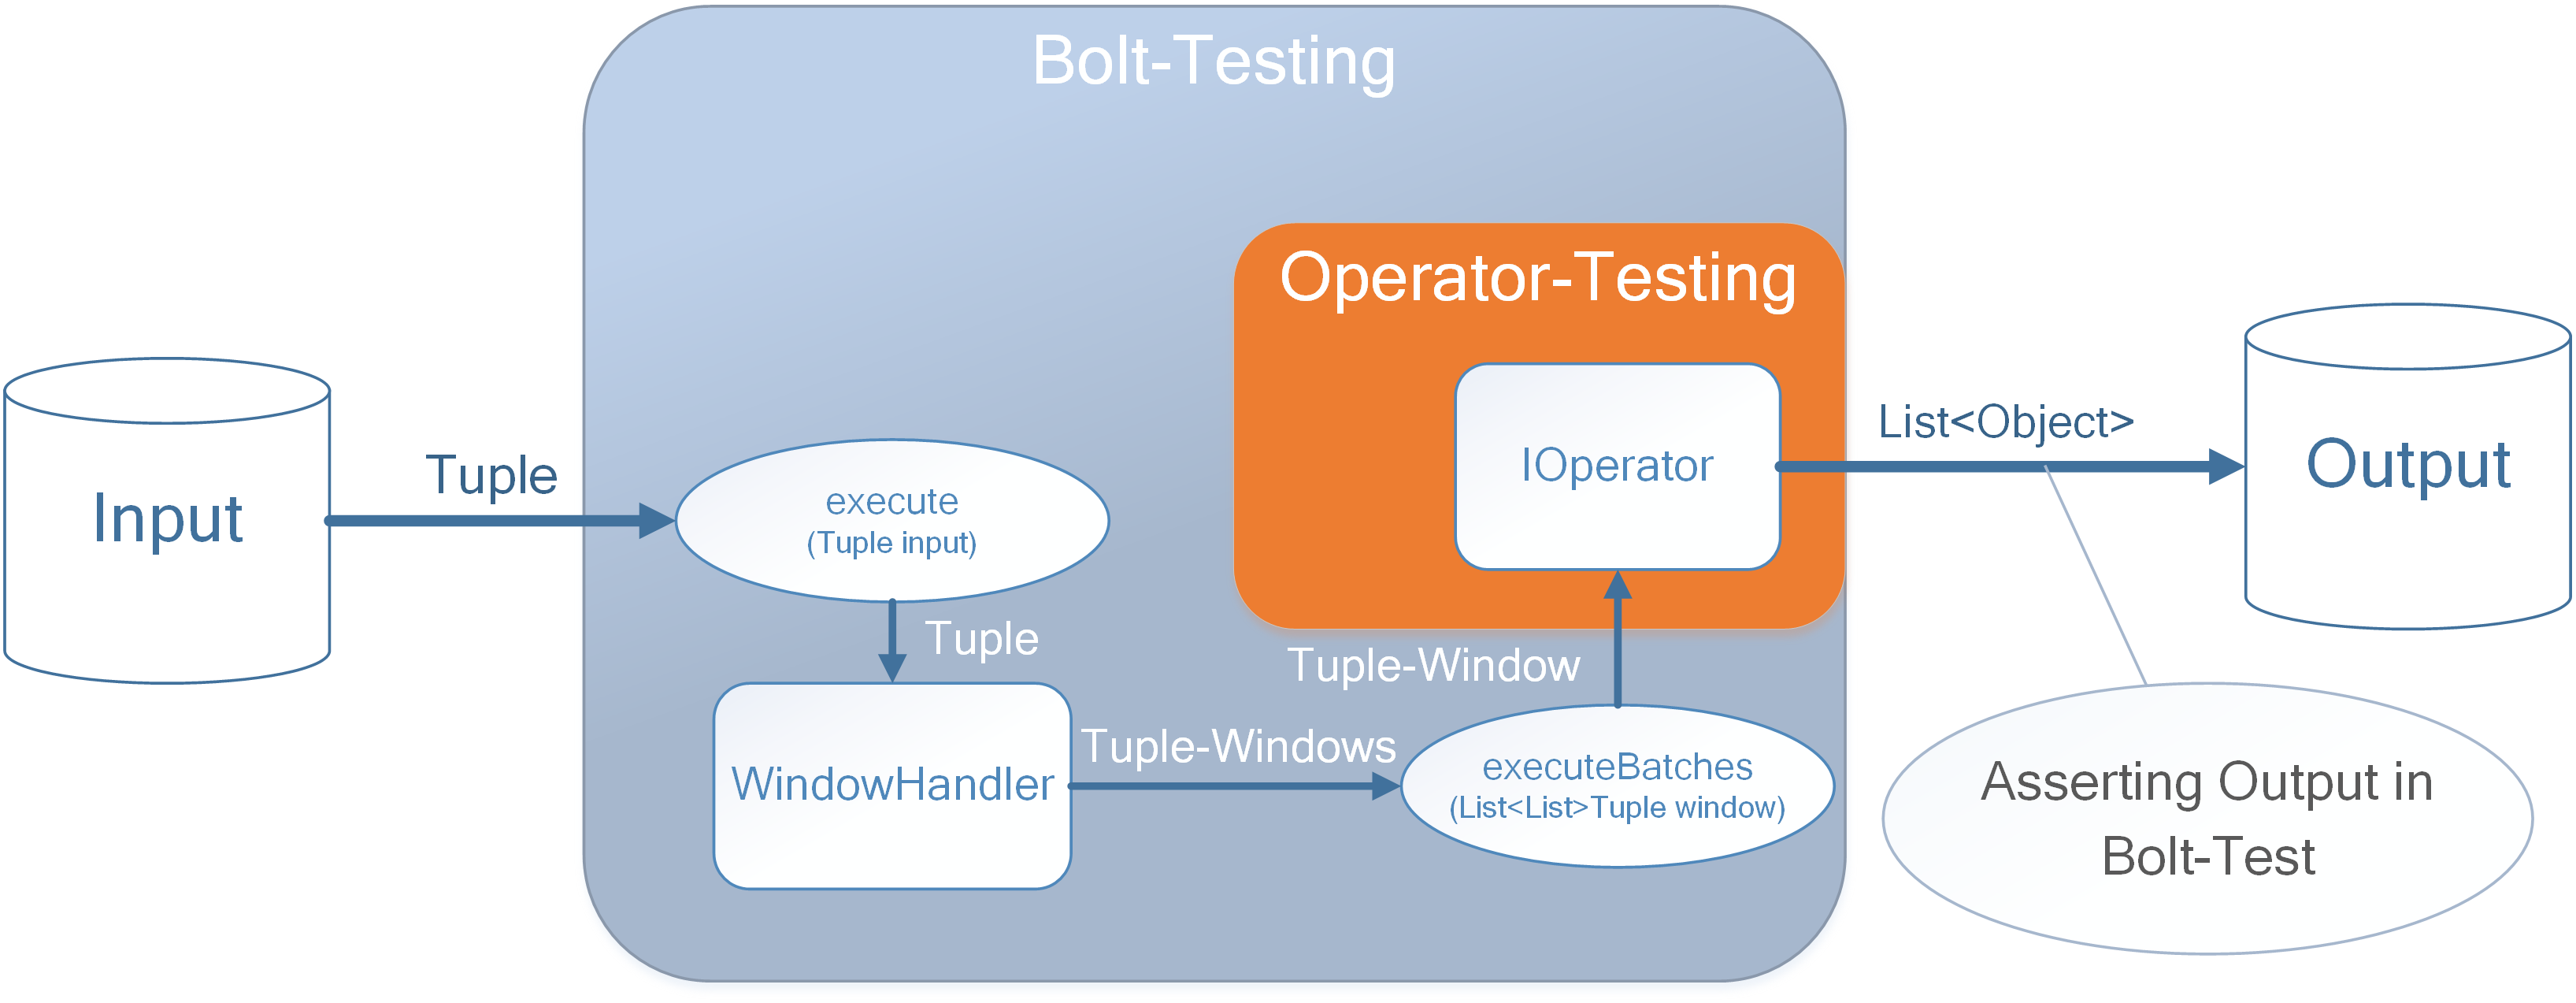
\includegraphics[width=0.4\textwidth]{./images/08_testing/BoltTests.png}
		\end{center}
	 
	 \descriptor{Topology-Tests}
		In order to test the topology as a whole, the Test-Suite provides a test skeleton named \texttt{TopologyTest}. A specific TopologyTest-Scenario is inherited by this class and allows the test-designer to test \textit{chains of Bolts with a Spout as source} in one run. Of course, this is not handling the complexity that Storm could cope with in its topologies, but as the Test-Suite is running outside a Storm environment (more on the implementation details may be found in the upcoming section \ref{sect:TestSuiteRealization}), it would be a likewise complex (and error-prone) task to completely simulate every aspect of Storm.\\
		The Topology-Test however does focus on linear topologies, which is describing most of the regular use-cases inside a Big-Data scenario. Even if the real Storm topology would use different Stream-Groupings (described in \ref{sect:StreamGroupings} on page \pageref{StreamGroupings}), the shuffled topology input could mostly be baked onto a linear topology. \\
		In order to set up a TopologyTest, import each Bolt from the topology to be tested into the test-class's \texttt{defineTopologySetup()} and add the respective Bolt in a \texttt{BoltTestConfig} in the order you want them to be placed in the testing chain. Each \texttt{BoltTestConfig} is carrying the respective \texttt{UDFBolt}, a Bolt-TestName, a timeout per tuple input (needed for \texttt{TimeWindows}) and an assertedOutput with it, in order to fully define a TopologyTest. The test run is then defined as an execution of different Bolt-Tests, initialized by the different \texttt{BoltTestConfigs}. Each Bolt-Test receives the output of the predecessing Bolt-Test as its own input. A Topology-Test could thus only succeed, if each Bolt-Test (and the Operator-Tests inside those) succeeds and on top of that, if the final output matches with the final asserted output of the topology, respective to the initial input.
		
		
	\end{description}

\subsection{Test-Suite Realization}
\label{sect:TestSuiteRealization}
	

\subsection{Treated Use-Cases}
\label{sect:TestSuiteUseCases}
	

\subsection{Test-Suite Limitations}
\label{sect:TestSuiteLimitations}
	